% figure1_hybrid.tex — Matrix + diamond operators in row gap.
% Same 2x3 grid as matrix variant, but with explicit operator shapes
% (compress, score) sitting between GPU and host rows.
% Shared preamble for standalone Figure 1 variants.
\documentclass[border=8pt,tikz]{standalone}
\usepackage{amsmath}
\usepackage{amssymb}
\usepackage{tikz}
\usetikzlibrary{arrows.meta,positioning,calc,fit,shapes.geometric,backgrounds}
\usepackage{xcolor}
\usepackage[T1]{fontenc}
\usepackage{mathptmx}
\newcommand{\repairkv}{\textsc{RepairKV}}
\newcommand{\bbase}{\ensuremath{B_{\mathrm{base}}}}
\newcommand{\bmatch}{\ensuremath{B_{\mathrm{match}}}}

\begin{document}
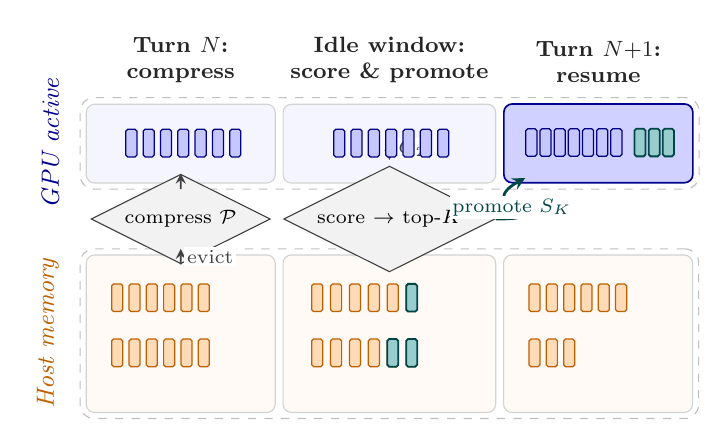
\begin{tikzpicture}[
  >=latex, line width=0.4pt,
  cell/.style={rounded corners=3pt, draw=gray!35},
  gpucell/.style={cell, fill=blue!4},
  hostcell/.style={cell, fill=orange!4},
  activecell/.style={cell, fill=blue!18, draw=blue!55!black, line width=0.6pt},
  op/.style={diamond, draw=black!75, fill=gray!10, inner sep=2pt,
             font=\scriptsize, align=center, aspect=2,
             minimum width=1.6cm, minimum height=0.55cm},
  chip/.style={rounded corners=0.7pt, minimum width=4pt, minimum height=10pt,
               inner sep=0pt, line width=0.45pt},
  gpuchip/.style={chip, draw=blue!50!black, fill=blue!22},
  hostchip/.style={chip, draw=orange!75!black, fill=orange!28},
  promchip/.style={chip, draw=teal!55!black, fill=teal!40, line width=0.65pt},
  rowband/.style={rounded corners=5pt, draw=gray!50, dashed, line width=0.4pt},
  bandlabel/.style={font=\itshape\small, text=black!70},
  collabel/.style={font=\bfseries\footnotesize, align=center, text=black!85},
  anno/.style={font=\scriptsize, text=black!72, align=center},
  arr/.style={->, line width=0.6pt, draw=black!75, >=stealth},
  promarr/.style={->, line width=1pt, draw=teal!55!black, >=stealth},
  arrlabel/.style={font=\scriptsize, fill=white, inner sep=1pt, text=black!75}
]
  \node[gpucell, minimum width=2.4cm, minimum height=1.0cm,
        anchor=south west] (gpu1) at (0, 1.9) {};
  \node[gpucell, minimum width=2.7cm, minimum height=1.0cm,
        anchor=south west] (gpu2) at (2.5, 1.9) {};
  \node[activecell, minimum width=2.4cm, minimum height=1.0cm,
        anchor=south west] (gpu3) at (5.3, 1.9) {};
  \node[hostcell, minimum width=2.4cm, minimum height=2.0cm,
        anchor=north west] (host1) at (0, 1.0) {};
  \node[hostcell, minimum width=2.7cm, minimum height=2.0cm,
        anchor=north west] (host2) at (2.5, 1.0) {};
  \node[hostcell, minimum width=2.4cm, minimum height=2.0cm,
        anchor=north west] (host3) at (5.3, 1.0) {};

  \begin{scope}[on background layer]
    \node[rowband, fit=(gpu1)(gpu3), inner xsep=2pt, inner ysep=2pt] (gband) {};
    \node[rowband, fit=(host1)(host3), inner xsep=2pt, inner ysep=2pt] (hband) {};
  \end{scope}
  \node[bandlabel, anchor=south, text=blue!55!black, rotate=90]
       at ([xshift=-4pt]gband.west) {GPU active};
  \node[bandlabel, anchor=south, text=orange!75!black, rotate=90]
       at ([xshift=-4pt]hband.west) {Host memory};

  \node[collabel, anchor=south] at ([yshift=4pt]gpu1.north)
       {Turn $N$:\\compress};
  \node[collabel, anchor=south] at ([yshift=4pt]gpu2.north)
       {Idle window:\\score \& promote};
  \node[collabel, anchor=south] at ([yshift=4pt]gpu3.north)
       {Turn $N{+}1$:\\resume};

  % Operators in row gap (diamonds)
  \node[op] (opcompress) at ($(gpu1.south)!0.5!(host1.north)$) {compress~$\mathcal{P}$};
  \node[op] (opscore)    at ($(gpu2.south)!0.5!(host2.north)$) {score $\to$ top-$K$};

  \draw[arr] ([yshift=-2pt]gpu1.south) -- (opcompress.north);
  \draw[arr] (opcompress.south) -- ([yshift=2pt]host1.north)
        node[arrlabel, midway, right=1pt] {evict};
  \draw[arr] ([yshift=10pt]opscore.north) -- ([yshift=2pt]opscore.north);
  \node[arrlabel, anchor=west] at ([xshift=2pt, yshift=6pt]opscore.north) {$Q_2$};

  % GPU chips
  \foreach \i in {1,...,7}{
    \pgfmathsetmacro{\xa}{0.22*\i+0.36}
    \pgfmathsetmacro{\xb}{0.22*\i+0.50}
    \pgfmathsetmacro{\xc}{0.18*\i+0.18}
    \node[gpuchip] at ([xshift=\xa cm,yshift=-0.5cm]gpu1.north west) {};
    \node[gpuchip] at ([xshift=\xb cm,yshift=-0.5cm]gpu2.north west) {};
    \node[gpuchip] at ([xshift=\xc cm,yshift=-0.5cm]gpu3.north west) {};
  }
  \foreach \i in {1,2,3}{
    \pgfmathsetmacro{\xs}{0.18*7+0.18*\i+0.30}
    \node[promchip] at ([xshift=\xs cm,yshift=-0.5cm]gpu3.north west) {};
  }

  % Host chips (2 sub-rows of 6)
  \foreach \i in {1,...,6}{
    \foreach \r in {0,1}{
      \pgfmathsetmacro{\xh}{0.22*\i+0.18}
      \pgfmathsetmacro{\yh}{-0.55-0.7*\r}
      \node[hostchip] at ([xshift=\xh cm,yshift=\yh cm]host1.north west) {};
    }
  }
  \foreach \i in {1,...,6}{
    \foreach \r in {0,1}{
      \pgfmathsetmacro{\xh}{0.24*\i+0.20}
      \pgfmathsetmacro{\yh}{-0.55-0.7*\r}
      \node[hostchip] at ([xshift=\xh cm,yshift=\yh cm]host2.north west) {};
    }
  }
  \pgfmathsetmacro{\xPa}{0.24*5+0.20} \pgfmathsetmacro{\yPa}{-0.55-0.7*1}
  \pgfmathsetmacro{\xPb}{0.24*6+0.20} \pgfmathsetmacro{\yPb}{-0.55-0.7*0}
  \pgfmathsetmacro{\xPc}{0.24*6+0.20} \pgfmathsetmacro{\yPc}{-0.55-0.7*1}
  \node[promchip] at ([xshift=\xPa cm,yshift=\yPa cm]host2.north west) {};
  \node[promchip] at ([xshift=\xPb cm,yshift=\yPb cm]host2.north west) {};
  \node[promchip] at ([xshift=\xPc cm,yshift=\yPc cm]host2.north west) {};
  \foreach \i in {1,...,6}{
    \pgfmathsetmacro{\xh}{0.22*\i+0.18}
    \node[hostchip] at ([xshift=\xh cm,yshift=-0.55cm]host3.north west) {};
  }
  \foreach \i in {1,...,3}{
    \pgfmathsetmacro{\xh}{0.22*\i+0.18}
    \node[hostchip] at ([xshift=\xh cm,yshift=-1.25cm]host3.north west) {};
  }

  % Promote (from score op to gpu3)
  \draw[promarr] (opscore.east)
        .. controls ($(opscore.east)+(0.8, 0)$)
                 and ($(gpu3.south west)+(-0.4, -0.3)$) ..
        ([xshift=8pt, yshift=2pt]gpu3.south west)
        node[arrlabel, text=teal!55!black, pos=0.55] {promote $S_K$};
\end{tikzpicture}
\end{document}
